\chapter{Avaliação}\label{ch:Avaliacao}

No âmbito científico, a avaliação de um determinado objeto de estudo busca, de modo geral, elucidar seu real impacto e influências sobre um determinado ambiente. O presente Capítulo apresenta os principais passos tomados para a avaliação do \acf{JS} desenvolvido pelo atual trabalho. Cada etapa influente para a efetiva avaliação do jogo desenvolvido é descrita nas demais seções. Desde modo, a \autoref{sec:Preparativos} descreve sobre os principais preparativos para a execução da pesquisa, a \autoref{sec:seg} fala sobre a segmentação da amostra, a \autoref{sec:pretes} apresenta os resultados alcançados na etapa de pré-teste, a \autoref{sec:tes} os resultados do teste, a \autoref{sec:postes} os resultados do pós-teste, a \autoref{sec:apreciar} descreve os resultados obtidos na etapa de apreciação e a \autoref{sec:compilar} compila os principais resultados, comparando-os com demais trabalhos na área. 

\section{Preparativos}\label{sec:Preparativos}

A corrente pesquisa realiza a avaliação do jogo \textbf{Infância Segura}, de modo a verificar se o jogo em si é capaz de cumprir com seus preceitos pré-estabelecidos. O principal preceito do jogo consiste na ideia de que o jogo é capaz de instruir crianças entre 5 (cinco) e 8 (oito) anos a reconhecerem eventos praticados (ou tentados) de violência sexual infantil. Para tal, se faz indispensável a busca por uma amostra de crianças (dentro da faixa etária estabelecida). O conselheiro tutelar Willians Odia e a assistente social Daniella Maragno prestaram seus conhecimentos para a atual pesquisa, elencando possíveis cenários de atuação. O intercâmbio de ideias levou a Escola Municipal Pauline Parucker (Joinville/\ac{SC}). Após algumas reuniões, a escola prestou seu parecer favorável, servindo de cenário para a execução da presente pesquisa. A diretora Rafaella de Sá Moreira Botelho e a supervisora Angela Marques de Liz Souza, são as principais agentes envolvidas no processo; processo esse, firmado oficialmente pela Declaração de Ciência e Concordância das Instituições Envolvidas (\autoref{chap:DIE}). 

A Escola Municipal Pauline Parucker, se dispôs a ceder um total 112 (cento e doze) crianças para a presente pesquisa, divididas em 4 (quatro) turmas: 2º Ano C, 2º Ano D, 3º Ano C, 3º Ano D. As crianças das turmas citadas foram convidadas a participar da pesquisa. Para as crianças interessadas em participar da pesquisa foram entregues dois termos, o Termo de Assentimento (\autoref{chap:TA}) e uma versão resumida do Termo de Consentimento Livre e Esclarecido (\autoref{chap:curto}). A versão resumida do Termo de Consentimento Livre e Esclarecido surge de modo a reduzir a quantidade de documentos físicos necessários, sem reduzir de fato, seus conteúdos, isso pois, a versão resumida apresenta um endereço que eletrônico que leva ao termo na íntegra (\autoref{chap:pagina}). Após um período de duas semanas, 33 (trinta e três) documentos retornaram: 8 (oito) do 2º Ano C, 12 (doze) do 2º Ano D, 10 (dez) do 3º Ano C e 3 (três) do 3º Ano D. Salienta-se que durante esse período, um vídeo explicativo sobre a pesquisa foi enviado pela escola (via \textit{WhatsApp}) aos guardiões legais das crianças. Por fim, enfatiza-se que todos os termos e protocolos foram publicados na Plataforma Brasil, os quais foram validados e aprovados pelo Comitê de Ética, sob o \ac{CAAE} nº 43602921.2.0000.0118.

%As crianças, em suas salas de aula e em horário escolar, são apresentadas à pesquisa. Após uma breve apresentação, os menores são convidados a participar da pesquisa. Para as crianças interessadas em participar da pesquisa são entregues duas vias de dois termos. Os termos entregues são o Termo de Assentimento e o Termo de Consentimento Livre e Esclarecido. É requisitado que as crianças apresentem tais termos aos seus guardiões legais, devendo retornar uma das vias de cada um dos termos para a escola. Só participam da corrente pesquisa as crianças com toda a documentação legal devidamente atestada. Visando garantir a integridade das assinaturas e fugir de falsificações cada assinatura é comparada ao documento de matrícula escolar assinado na escola presencialmente pelos pais/responsáveis de cada criança. Todos os termos e declarações do presente estudo são impressos em duas vias. A presente pesquisa se compromete a manter guardada uma das vias por um período de 5 (cinco) anos, assim como todos os registros e resultados alcançados. O término da coleta de toda a documentação legal demarca o início do processo de segmentação da corrente pesquisa. 


\section{Segmentação}\label{sec:seg}

Ao total, 33 (trinta e três) crianças apresentaram toda a documentação necessária para participar na corrente pesquisa. Uma vez estabelecida a quantidade de indivíduos aptos a participar no corrente estudo, iniciou-se o processo de segmentação da amostra. 

A amostra foi segmentada em dois grupos: Grupo Controle e Grupo Experimental. A segmentação resultou em um grupo controle composto por 18 (dezoito) crianças e um grupo experimental composto por 15 (quinze) crianças. A disposição detalhada dos grupos ficou da seguinte maneira: grupo controle com 8 (oito) crianças do 2º Ano C e 10 (dez) crianças do 3º Ano C e grupo experimental com 12 (doze) crianças do 2º Ano D e 3 (três) crianças do 3º Ano D.


\section{Pré-teste}\label{sec:pretes}

A etapa de pré-teste do atual trabalho foi realizada no dia 19 (dezenove) de outubro de 2021 às 13h30 (hora local). A etapa de pré-teste surge na presente pesquisa com o objetivo de identificar, a existência ou não, de diferenças significativas entre o grupo controle e grupo experimental, no que diz respeito aos seus conhecimentos sobre abuso infantil. A medição dos conhecimentos das crianças é feita com auxílio do instrumento avaliativo \acf{CKAQ} adaptado ao português (\autoref{chap:traduzido}). 

A etapa de pré-teste ocorreu em dois momentos, inicialmente com as turmas do 3º (terceiro) Ano na biblioteca da escola e posteriormente com as turmas do 2º (segundo) Ano em uma sala de aula tradicional. O processo do pré-teste foi inteiramente realizado pelo presente autor com acompanhamento da supervisora Angela Marques de Liz Souza, sendo ela a responsável pela separação e remanejamento das turmas, conforme o regimento escolar. À todas as crianças foi entregue uma cópia impressa do \ac{CKAQ} adaptado ao português. Após a entrega, breves instruções sobre seu conteúdo e sua forma de preenchimento foram passadas (\autoref{chap:teste}). %(semelhante ao \autoref{chap:teste}). Qualquer dúvida poderia ser respondia com a criança levantando a mão.

O questionário foi lido em voz alta às crianças. O número da questão era lido, juntamente com seu pictograma representativo para situar as crianças sobre a pergunta corrente do questionário que deveria ser assinalada. Uma questão por vez era lida e relida, fornecendo em seguida, uma janela de tempo para as crianças deliberarem e responderem a questão. Nesse intervalo de tempo, as crianças eram indagadas se concordavam ou se discordavam do que havia sido lido, ou seja, se elas achavam verdade ou mentira a última questão lida. Para apoiar esse processo foram realizados gestos de positivo e negativo com as mãos.

O atual estudo não se dispôs a ceder material para o preenchimento do questionário (como lápis e borracha). As crianças participantes, utilizaram seus próprios materiais escolares para assinalar as questões do questionário. O processo como um todo contou com a participação de 31 (trinta e uma) crianças e durou uma hora e trinta minutos, finalizando às 15h (hora local). Cada momento de aplicação teve duração de quarenta e cinco minutos, com duas crianças faltantes do grupo controle (uma de cada turma). Ao término, as crianças retornaram a sua agenda escolar sem demais prejuízos. Por fim, os questionários foram recolhidos e levados para análise.

A análise dos dados do questionário visa compreender melhor o conhecimento de ambos os grupos no que tange os assuntos ministrados pelo questionário em si. Dentre as informações que podem ser coletados por essa análise, está a taxa de acerto por questão. Questões em branco ou rasuradas (de difícil identificação) são consideradas erradas. A corrente pesquisa computou um total de 26 (vinte e seis) questões que haviam sido deixadas em branco ou rasuradas. A taxa de acerto por questão do grupo controle pode ser observada na \autoref{fig:barrasCon}.

\begin{figure}[htb]

    \caption{\label{fig:barrasCon}Taxa de acerto por questão, pré-teste (grupo controle).}
    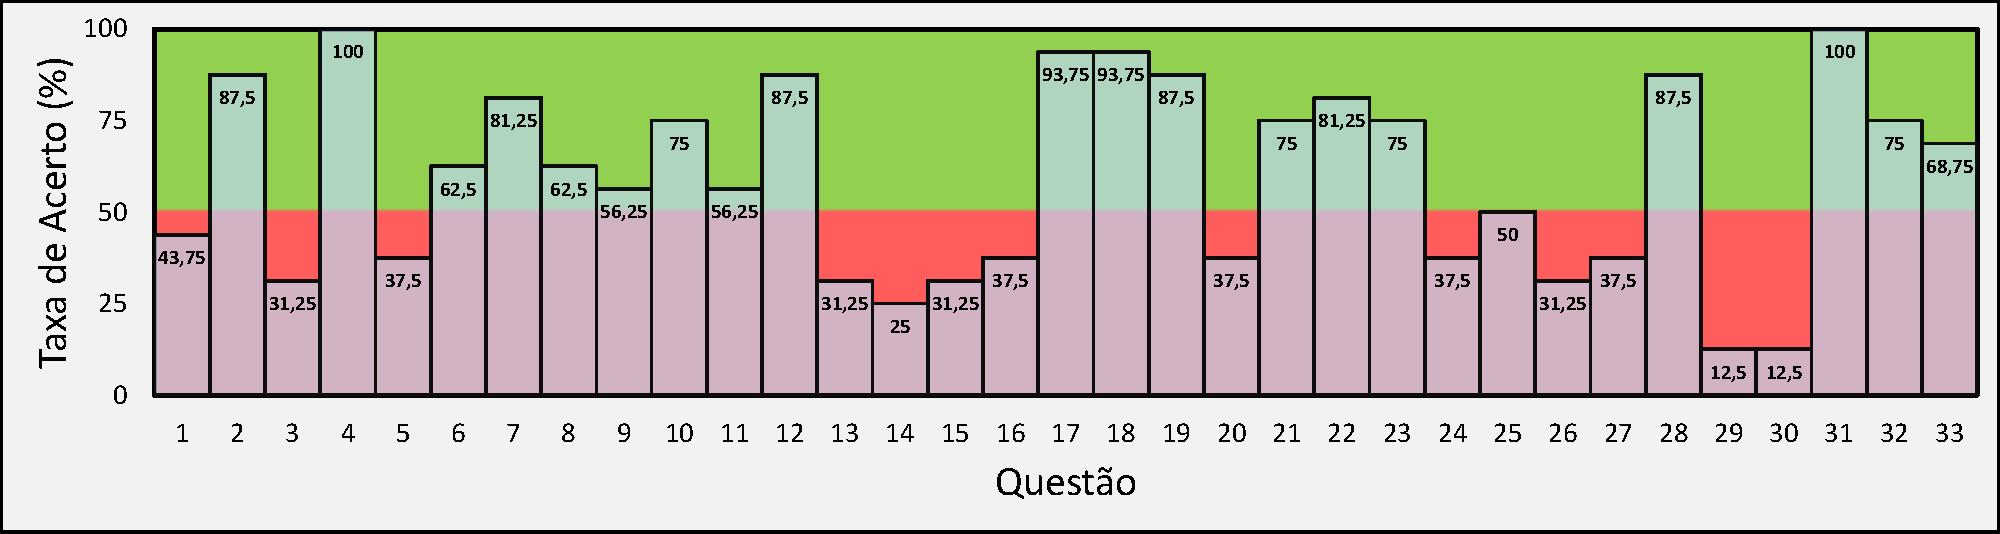
\includegraphics[width=\linewidth]{./Visuais/Notas4.pdf}
    \legend{Fonte: Elaborada pelo autor (2021).}
  
\end{figure}

A \autoref{fig:barrasCon} ilustra a taxa de acerto por questão (grupo controle). O eixo das abscissas representa cada uma das questões do questionário, sendo o número 1 (um) a primeira questão do questionário e o número 33 (trinta e três) a última questão do questionário. O eixo das ordenadas representa a taxa de acerto, indo de 0 (zero) a 100 (cem). O número 0 (zero) significa que nenhum indivíduo acertou aquela questão, o número 100 (cem) significa que todos os indivíduos acertaram aquela questão. No presente caso, tanto a questão 4 (quatro), quanto a questão 31 (trinta e um), tiveram uma taxa de acerto de 100\% para o grupo controle. O mesmo não ocorre com o grupo experimental como pode ser observado na \autoref{fig:barrasExp}.

\begin{figure}[htb]

    \caption{\label{fig:barrasExp}Taxa de acerto por questão, pré-teste (grupo experimental).}
    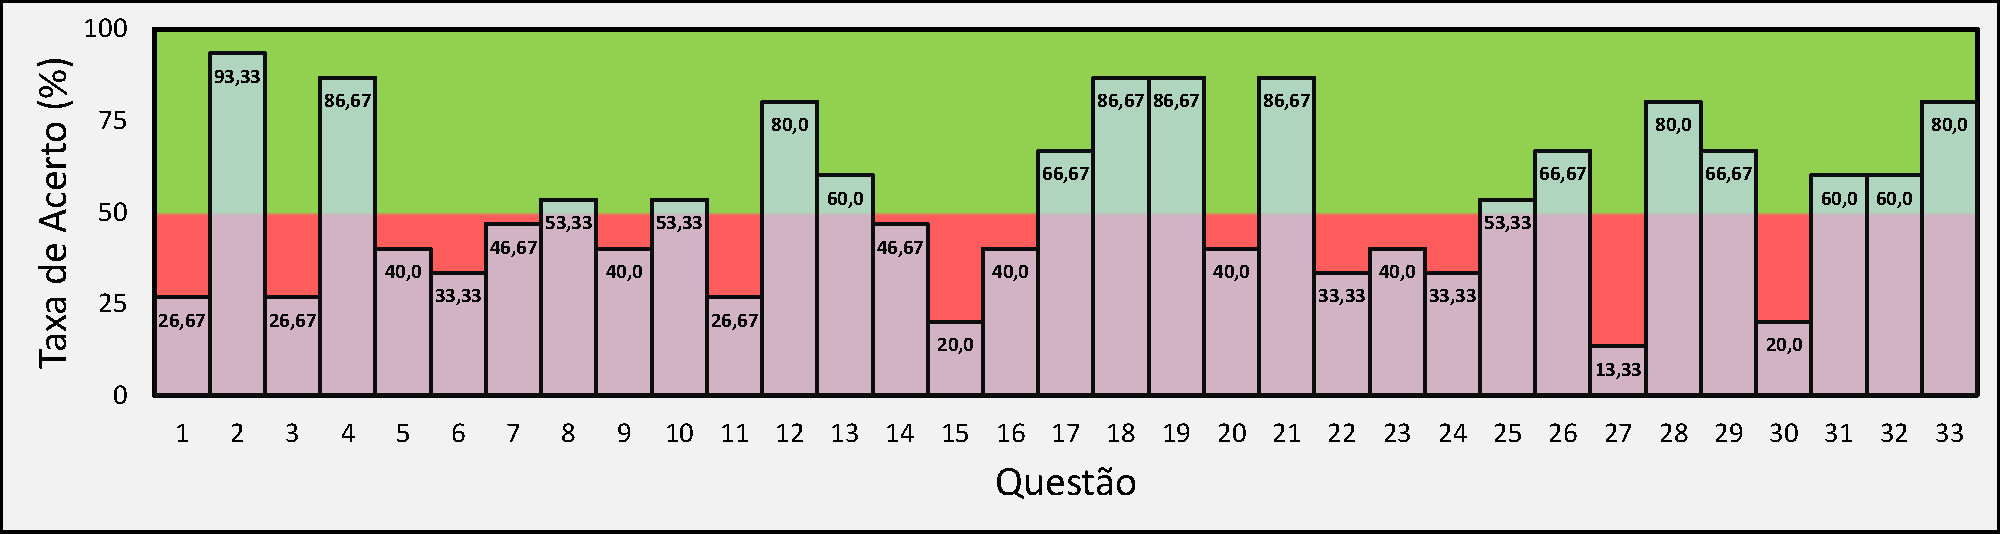
\includegraphics[width=\linewidth]{./Visuais/Notas3.pdf}
    \legend{Fonte: Elaborada pelo autor (2021).}
  
\end{figure}

A \autoref{fig:barrasExp} apresenta a taxa de acerto por questão (grupo experimental). Em comparação ao grupo controle (\autoref{fig:barrasCon}) o grupo experimental teve um desempenho ligeiramente inferior. Buscando fornecer um panorama melhor dos resultados alcançados nessa etapa, produziu-se um diagrama de caixa estreita (\autoref{fig:caixaprePRE}).

\begin{wrapfigure}[15]{r}{9.0cm}%pulando 15 linhas
    \vspace{-4pt}
    \caption{\label{fig:caixaprePRE}Diagrama geral das notas, pré-teste.}
    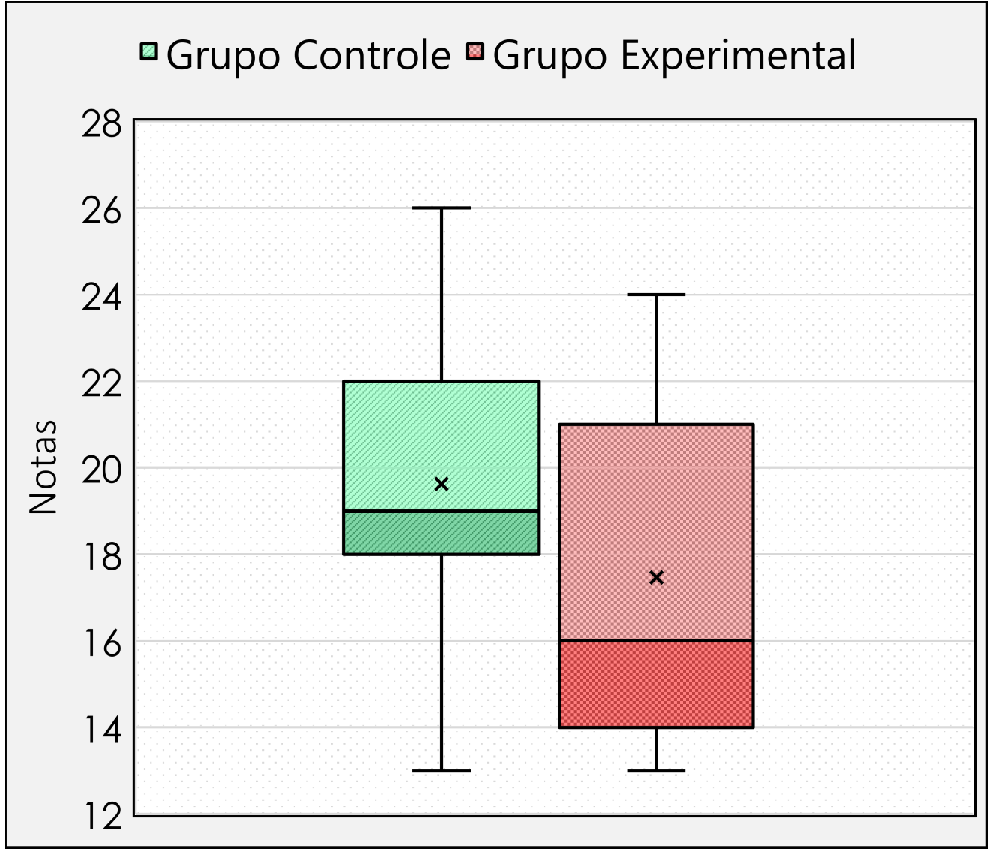
\includegraphics[width=\linewidth]{./Visuais/CaixaEstreitaEnfeitado.pdf}
    \legend{Fonte: Elaborada pelo autor (2021).}
\end{wrapfigure}

Um diagrama de caixa mostra a distribuição dos dados em quartis, realçando a média e as exceções. No caso do presente estudo o grupo controle acertou em média 19,625 ($\sigma$ = 3,18) questões (59,47\%, $\sigma$ = 9,64), enquanto o grupo experimental acertou em média 17,467 ($\sigma$ = 3,96) questões (52,93\%, $\sigma$ = 12), valores representados pela marcação em $\times$ na \autoref{fig:caixaprePRE}. A maior quantidade de acertos foi de 26 (vinte e seis) questões no grupo controle e 24 (vinte e quatro) questões no grupo experimental. Ambos os grupos tiveram uma menor quantidade de acertos de 13 (treze) questões.

A análise feita das amostras serve de apoio para uma compreensão básica dos grupos estudados, todavia os cálculos realizados não são suficientes para alcançar conclusões mais robustas. Além de calcular tais valores, é preciso interpretá-los estatisticamente. Por tanto, para a devida condução da atual pesquisa é necessário interpretar se há equivalência ou diferença estatística entre as amostras. Nesse sentido, a estatística possui um conjunto de testes para averiguar o grau de equivalência entre duas amostras. %Alguns testes estatíticos necessitam que determinados critérios sejam cumpridos para que o teste em si seja realizado sem erros. 

O presente estudo se utiliza de dois testes estatísticos, um para calcular a média ($\overline{\times}$) e outro para calcular a mediana ($\tilde{\times}$). Para o cálculo da mediana o corrente trabalho acadêmico se utilizou do teste de \textit{Mann-Whitney}. O teste compara duas amostras independentes, de modo a calcular se há equivalência entre suas medianas. Dito isso, o atual estudo fez uso do teste de \textit{Mann-Whitney} para determinar, a existência ou não, de equivalência entre as medianas do grupo controle e do grupo experimental. Os cálculos apontaram para uma equivalência entre as amostras (U = 64; p = 0,08323). Desta forma a hipótese nula (H$_0$) do teste de \textit{Mann-Whitney} deve ser aceita, indicando que as medianas entre os grupos são equivalentes (\textit{M}$_{controle}$ = \textit{M}$_{experimental}$). %com 95\% de confiança de

Para o cálculo da média o presente estudo se utilizou do Teste \textit{t}. O Teste \textit{t} é considerado exato e adequado para a hipótese de igualdade de médias. No entanto, o Teste \textit{t} exige que alguns critérios sejam cumpridos para que seus resultados tenham validade estatística. Um destes critérios exige que os dados das amostras devem obedecer uma distribuição normal. Nesse sentido, a presente pesquisa se utilizou de dois testes de normalidade, o teste de \textit{Shapiro-Wilk} e o teste de \textit{D'Agostino-Pearson}, ambos indicaram que  os dados colhidos obedecem uma distribuição normal. Outro critério exigido pelo Teste \textit{t} diz respeito a variância das amostras. Os cálculos realizados indicaram que as variâncias do grupo controle e grupo experimental são equivalentes ($\alpha$ = 5\%). Deste modo, o Teste \textit{t} pode ser realizado, concluindo ao final que as amostras são de fato, equivalentes ($\alpha$ = 5\%). A \autoref{fig:normal} ilustra a equivalência entre as amostras. 

\begin{figure}[htb]
    \centering
    \caption{\label{fig:normal}Distribuição das notas atingidas, pré-teste.}
    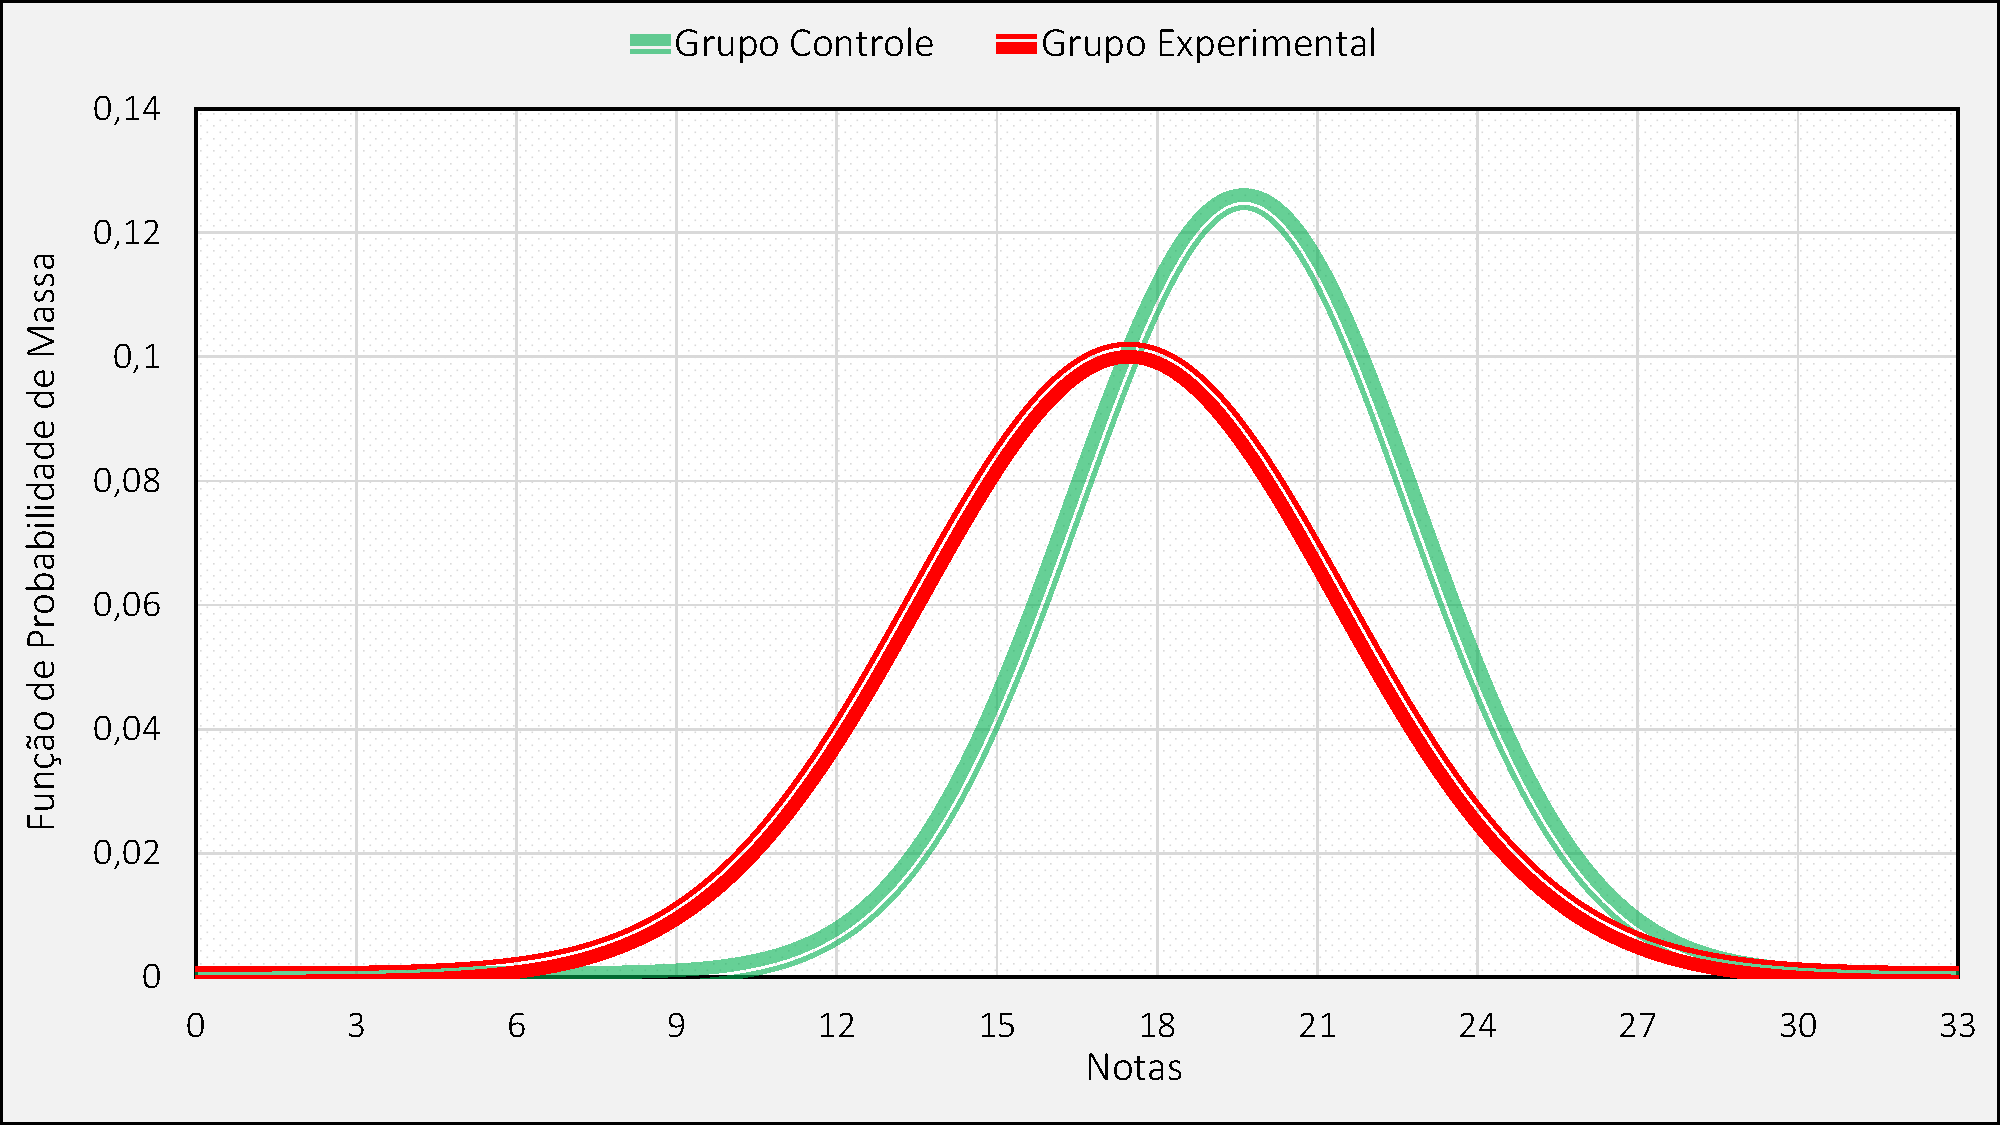
\includegraphics[width=\linewidth]{./Visuais/Graficos1.pdf}
    \legend{Fonte: Elaborada pelo autor (2021).}
  
\end{figure}

A \autoref{fig:normal} ilustra as distribuições normais do grupo controle e do grupo experimental. O eixo das abscissas representa o total de acertos no questionário, indo de 0 (zero) até 33 (trinta e três), tal escala indica a quantidade de questões assinaladas corretamente no questionário. Já o eixo das ordenadas representa a probabilidade da quantidade de acertos. Os máximos globais de cada grupo, são as médias já calculadas e ilustradas na \autoref{fig:caixaprePRE}.

O Teste \textit{t} mostrou que não há diferenças significativas entre as médias das amostras (t$_{(27)}$ = 1,655; p = 0,10953). Ou seja, os resultados do Teste \textit{t} indicam não haver diferenças de conhecimento entre as crianças do grupo controle e as crianças do grupo experimental, no que diz respeito aos conhecimentos medidos pelo instrumento avaliativo \ac{CKAQ}. Desta forma a hipótese nula (H$_0$) do Teste \textit{t} deve ser aceita, indicando que não existe diferenças entre as médias das amostras ($\mu$$_{controle}$ = $\mu$$_{experimental}$). 

Os resultados alcançados nessa seção apontam; tanto para uma média, quanto para uma mediana, equivalente entre as amostras. Notoriamente, os cálculos matemáticos realizados pela presente pesquisa não estão isentos de falhas, portanto, com intuito de facilitar a revisão dos resultados alcançados, e com intuito de deixar todo o processo mais transparente o possível a corrente pesquisa publica todos os dados obtidos nessa etapa no \autoref{chap:resul1}.

Por fim, é importante salientar que os resultados alcançados na etapa de pré-teste da atual pesquisa correspondem aos resultados esperados para essa etapa. Isso pois, o corrente trabalho, só poderia prosseguir com a pesquisa caso as amostras estudadas fossem equivalentes. Sendo as amostras equivalentes, o jogo desenvolvido pelo atual trabalho pode então, ser aplicado ao grupo experimental na etapa de teste da corrente pesquisa (\autoref{sec:tes}).


\section{Teste}\label{sec:tes}

A etapa de teste do atual trabalho ocorreu em três momentos distintos; dia 3 (três), dia 4 (quatro) e dia 5 (cinco) de novembro de 2021. No dia 3 (três) foram realizados os preparativos para a instalação do jogo nos \textit{tablets} da escola (modelo \textit{Multilaser} M10A). O processo se iniciou às 14h e terminou às 16h15 (hora local). O processo de instalação do jogo nos \textit{tablets} se deu na biblioteca da escola e contou com a participação da professora Carla Diacui Medeiros Berkenbrock, a supervisora Angela Marques de Liz Souza e o presente autor desta dissertação. Ao total o jogo foi instalado em 30 (trinta) \textit{tablets}. Foi realizada a instalação do jogo em mais \textit{tablets} do que o necessário, visando contornar demais empecilhos como problemas ou falta de energia em algum determinado dispositivo durante a etapa de teste (apenas um \textit{tablet} foi trocado durante os experimentos). %Ao final, todos os \textit{tablets} foram colocados em um gabinete de recarga.

Nos dias 4 (quatro) e 5 (cinco) de novembro de 2021 a presente pesquisa conduziu sua etapa de teste com crianças (na bilioteca da escola). O processo consistiu em submeter aos participantes (crianças), o objeto estudado (jogo). No dia 4 (quatro) as crianças participantes foram instruidas a jogar o jogo \textbf{Infância Segura}, mais especificamente as fases sobre \textbf{Direitos} (\autoref{subsec:2}) e \textbf{Denúncias} (\autoref{subsec:3}). No dia 5 (cinco) as crianças foram instruidas a jogar as demais fases, sobre \textbf{Anatomia} (\autoref{subsec:1}) e \textbf{Redes Sociais} (\autoref{subsec:4}). Essa separação das fases foi uma sugestão da supervisora Angela. É importante salientar que a etapa de teste foi conduzida inteiramente e apenas com as crianças do grupo experimental, com uma criança do 3º Ano D faltante no dia 5 (cinco). Em ambos os dias o processo se iniciou às 13h40.

No dia 4 (quatro) e no dia 5 (cinco) os \textit{tablets} foram distribuídos sobre as mesas da biblioteca da escola. As crianças foram entrando, duas a duas, na biblioteca da escola, sendo instruídas a sentarem na frente do \textit{tablet} que contivesse uma etiqueta com seu nome escrito (no último dia a posição dos \textit{tablets} foi trocada). Em ambos os dias as crianças tiveram contato com o jogo por quarenta e cinco minutos, totalizando ao total uma hora e trinta minutos de atividades (com início às 14h15 e término às 15h). O processo foi inteiramente conduzido pelo presente autor desta dissertação, com auxílio da supervisora Angela (todos os dias). Em separado, no 4 (quatro) a pesquisadora responsável Carla Diacui Medeiros Berkenbrock e no dia 5 (cinco) a aposentada Rocilda Cordeiro Mendonça, prestaram sua atenção e auxílio a pesquisa. Em específico a supervisora Angela foi a responsável pelo remanejamento dos estudantes. %Em específico a suprevisora Angela foi a responsável por remanejar os estudantes das suas salas à biblioteca (e vice-versa).

No primeiro dia, as crianças foram apresentadas ao jogo com auxílio de um projetor. Neste momento as crianças foram instruídas a se identificarem no jogo e a informarem seu gênero. As crianças também foram instruídas a como alterar o volume do jogo e a como intercambiar entre as fases. No segundo dia, com auxílio do mesmo projetor, realizou-se uma revisão do terceiro minijogo da fase sobre \textbf{Direitos} e do primeiro minijogo da fase sobre \textbf{Redes Sociais}. Tais minijogos foram escolhidos para uma revisão, uma vez observado que os conteúdos contidos nestes minijogos coincidiam com os conteúdos das questões com menores taxas de acerto para o grupo experimental na etapa de pré-teste (\autoref{sec:pretes}).

No segundo dia, as crianças (em geral) apresentaram muita dificuldade para concluir o primeiro e o segundo minijogo da fase sobre \textbf{Anatomia}. Em virtude dessa dificuldade, instruções mais detalhadas de cada minijogo foram passadas com auxílio de um projetor. Por fim, a taxa de conclusão do jogo (quatro fases) ficou em 89,63\%. Ao todo 7 (sete) crianças deixaram de concluir uma ou mais fases no jogo. Os minijogos da etapa de \textbf{Direitos} e \textbf{Redes Sociais} foram os minijogos com melhor desempenho entre os jogadores. Seguidos pelos minijogos da etapa de \textbf{Denúncias} e pelos minijogos da etapa de \textbf{Anatomia}, com os piores desempenhos. 

No segundo dia, a rede sem fio da escola apresentou instabilidade. Tal instabilidade impossibilitou que os dados dos estudantes (gerados durante o jogo) fossem enviados aos servidores da aplicação. No entanto, os dados gerados pelos jogadores durante a etapa de teste, além de estarem programados para serem enviados a um banco de dados, também estavam programados para armazenar todo conjunto de ações dos seus jogadores localmente (nos \textit{tablets}). Com isso, após o fim dos experimentos no segundo dia, o conteúdo de cada jogador foi extraído dos \textit{tablets} (o processo levou em torno de uma hora). Por fim, a etiqueta dos tablet foi removida, os \textit{tablets} foram desligados e colocados em um gabinete de recarga. Ao total, 3.315 ações foram computadas nos minijogos, dando em média, 221,83 ações por jogador.

Durante a etapa de teste, nenhum dos envolvidos manifestou qualquer quadro de angústia, nervosismo, ansiedade ou constrangimento para com os conteúdos abordados pelo jogo. Destaca-se apenas que, uma das crianças, apresentou sinais de preocupação, ao sentir que estava demorando mais do que os seus outros colegas para concluir os minijogos. Também destaca-se que, algumas crianças, tiveram dificuldades em compreender os diálogos do jogo, pedindo muitas vezes, para que os diálogos fossem lidos para elas. O fato de muitas crianças não estarem plenamente alfabetizadas, acabou por atrapalhar a absorção do conteúdo pelas crianças. Isso pois, por mais que o jogo estivesse localizado em português, a execução conjunta  dos \textit{tablets} em um mesmo ambiente acabou gerando um certo ruído sonoro no ambiente, dificultando os áudios de serem ouvidos. As crianças levantavam suas mãos quando necessitavam de alguma ajuda ou auxílio, quando precisavam ir ao banheiro ou quando gostariam de informar que concluíram com todo o conteúdo. As crianças que manifestaram terem concluído todo o jogo foram liberadas a jogar qualquer minijogo de seu interesse (até o término das atividades). 

O jogo em si apresentou algumas falhas de desenvolvimento durante a etapa de teste. Nesse sentido, falhas tanto técnicas, quanto conceituais foram constatadas. Tais observações geraram ideias de aperfeiçoamento e melhorias, as quais foram manifestadas pelos profissionais envolvidos na corrente pesquisa. Tais ideias são descritas no \autoref{ch:Conclusao} do presente trabalho acadêmico, de modo a compilar conjuntamente as ideias manifestadas pelas crianças do grupo experimental. 

 
\section{Pós-teste}\label{sec:postes}

A etapa de pós-teste do corrente trabalho foi conduzida no dia 22 (vinte e dois) de novembro de 2021 às 13h50 (hora local). A etapa de pós-teste surge na presente pesquisa com o objetivo de identificar, a existência ou não, de diferenças significativas entre o grupo controle e grupo experimental, no que diz respeito aos seus conhecimentos sobre abuso infantil. A medição dos conhecimentos das crianças é feita com auxílio do instrumento avaliativo \acf{CKAQ} adaptado ao português (\autoref{chap:traduzido}). 

A etapa de pós-teste ocorreu em dois momentos, inicialmente com o grupo experimental na biblioteca da escola e posteriomente com o grupo controle em uma sala de aula tradicional. O processo do pós-teste foi inteiramente realizado pelo presente autor com acompanhamento da pesquisadora responsável Carla Diacui Medeiros Berkenbrock e da supervisora Angela Marques de Liz Souza, sendo ela a responsável pela separação e remanejamento das turmas, conforme o regimento escolar. À todas as crianças foi entregue uma cópia impressa do \ac{CKAQ} adaptado ao português. Após a entrega, breves instruções sobre seu conteúdo e sua forma de preenchimento foram passadas (\autoref{chap:teste}).

O questionário foi lido em voz alta as crianças. O número da questão era lido, juntamente com seu pictograma representativo para situar as crianças sobre a pergunta corrente do questionário que deveria ser assinalada. Uma questão por vez era lida e relida, fornecendo em seguida, uma janela de tempo para as crianças deliberarem e responderem a questão. Nesse intervalo de tempo, as crianças eram indagadas se concordavam ou se discordavam do que havia sido lido, ou seja, se elas achavam verdade ou mentira a última questão lida. Para apoiar esse processo foram realizados gestos de positivo e negativo com as mãos.

O presente estudo não se dispôs a ceder material para o preenchimento do questionário (como lápis e borracha). As crianças participantes, utilizaram seus próprios materiais escolares para assinalar as questões do questionário. O processo como um todo contou com a participação de 29 (vinte e nove) crianças e durou uma hora (com término às 14h20 para o grupo experimental e às 16h30 com o grupo controle). Cada momento de aplicação do questionário teve duração de trinta minutos, com quatro crianças faltantes (uma de cada turma). Ao término, as crianças do grupo controle retornaram a sua agenda escolar sem demais prejuízos, já as crianças do grupo experimental passaram por uma etapa a mais da corrente pesquisa, a qual é descrita mais detalhadamente no \autoref{sec:apreciar}. Todavia, antes de dar andamento para a próxima etapa da pesquisa, é preciso analisar e interpretar os dados gerados na presente etapa. 

Após a coleta e análise dos questionários a corrente pesquisa computou um total de 7 (sete) questões deixadas em branco ou rasuradas. Tal como na etapa de pré-teste (\autoref{sec:pretes}) a etapa de pós-teste também compila as taxas de acerto por questão do grupo controle e do grupo experimental, permitindo assim, uma comparação mais detalhada e acurada entre os desenvolvimentos internos de cada grupo. A taxa de acerto por questão do grupo controle pode ser observada na  \autoref{fig:barrasCon1}.


\begin{figure}[htb]

    \caption{\label{fig:barrasCon1}Taxa de acerto por questão, pós-teste (grupo controle).}
    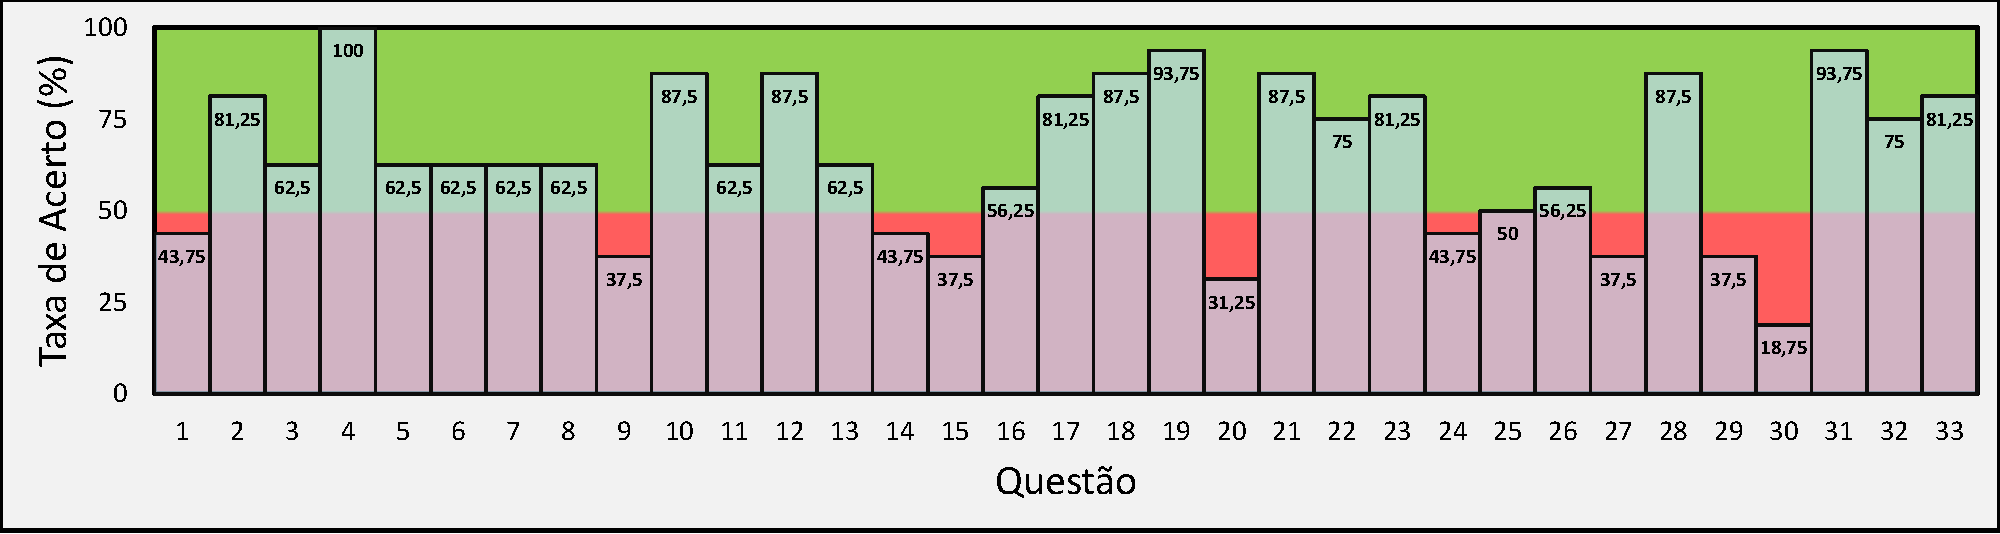
\includegraphics[width=\linewidth]{./Visuais/NotasControlePOS.pdf}
    \legend{Fonte: Elaborada pelo autor (2021).}
  
\end{figure}

A \autoref{fig:barrasCon1} revela que as crianças do grupo controle mantiveram uma taxa de acerto de 100\% para a questão 4 (quatro), todavia em relação ao pré-teste, as crianças não mantiveram o mesmo desempenho para a questão 31 (trinta e um). Em síntese observou-se uma ligeira evolução de desempenho entre o pré e o pós-teste. Ao total 16 (dezesseis) questões foram computadas com um desempenho superior ao constatado na etapa de pré-teste para o grupo controle. 
%As questões que tiveram um desempenho superior são as questões: 3, 5, 10, 11, 13, 14, 15, 16, 19, 21, 23, 24, 26, 29, 30, 33
No entanto, um desempenho mais acentuado é observado no grupo experimental como ilustra o gráfico em barras da \autoref{fig:barrasExp1}.


\begin{figure}[htb]

    \caption{\label{fig:barrasExp1}Taxa de acerto por questão, pós-teste (grupo experimental).}
    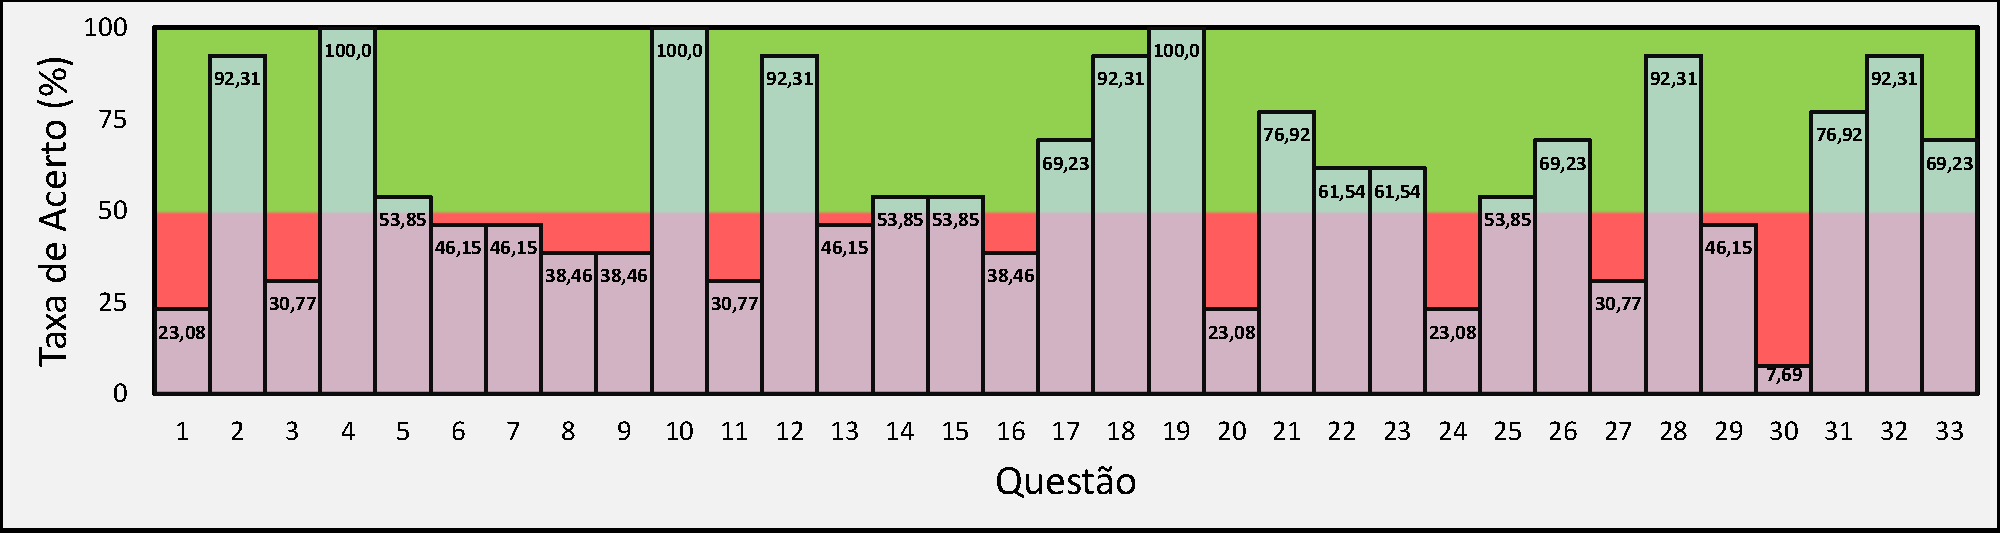
\includegraphics[width=\linewidth]{./Visuais/NotasExperimentalPOS.pdf}
    \legend{Fonte: Elaborada pelo autor (2021).}
  
\end{figure}

A \autoref{fig:barrasExp1} revela que as crianças do grupo experimental tiveram uma taxa de acerto de 100\% para a questão 4 (quatro), 10 (dez) e 19 (dezenove).  Em síntese observou-se uma evolução de desempenho entre o pré e o pós-teste do grupo experimental. Ao total 20 (vinte) questões foram computadas com um desempenho superior ao constatado na etapa de pré-teste.
%As questões que tiveram um desempenho superior são as questões: 3, 4, 5, 6, 10, 11, 12, 14, 15, 17, 18, 19, 22, 23, 25, 26, 27, 28, 31, 32.
As crianças do grupo experimental manifestam um progresso mais expressivo de desempenho quando comparadas com o grupo controle. Todavia, a evolução interna dos grupos não se destaca, quando as amostras são comparadas entre si. Nesse sentido, para fornecer um panorama melhor dos resultados alcançados nessa etapa da pesquisa, produziu-se um diagrama de caixa estreita, ilustrado na \autoref{fig:caixapre1}.

\begin{wrapfigure}[15]{r}{9.0cm}%pulando 15 linhas
    \vspace{-4pt}
    \caption{\label{fig:caixapre1}Diagrama geral das notas, pós-teste.}
    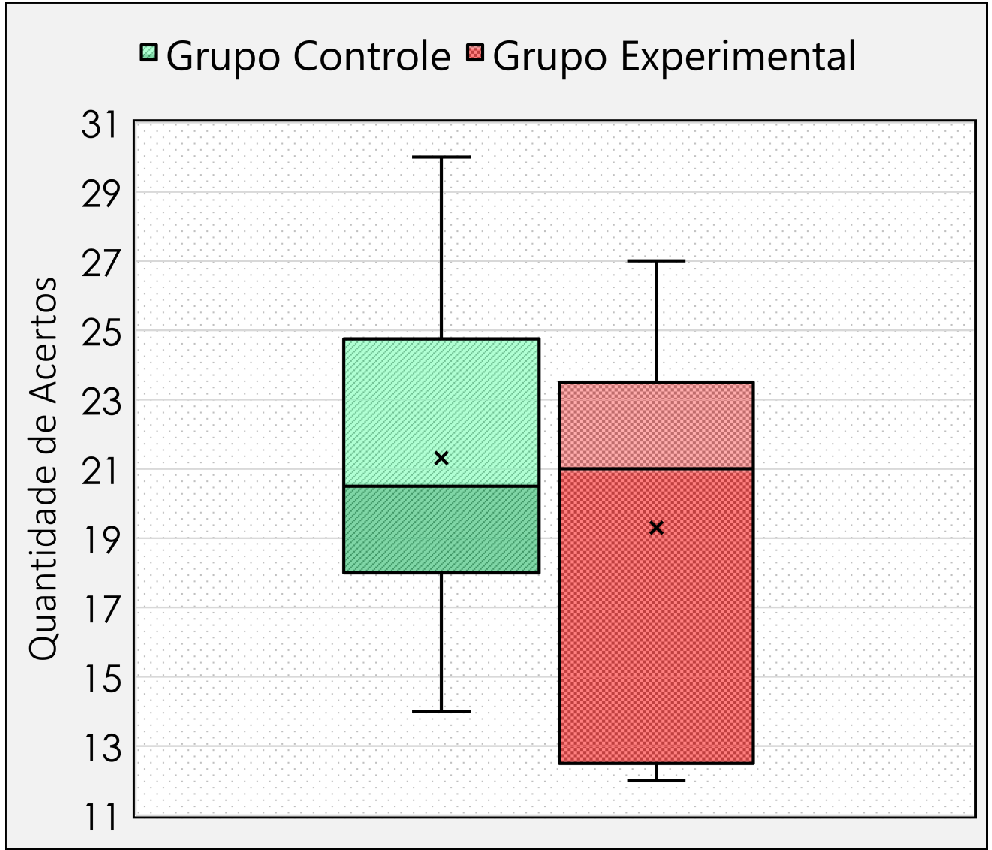
\includegraphics[width=\linewidth]{./Visuais/CaixaEstreitaPOS.pdf}
    \legend{Fonte: Elaborada pelo autor (2021).}
\end{wrapfigure}

Os resultados do diagrama de caixa estreita mostram que o grupo controle teve uma taxa de acerto média 21,312 ($\sigma$ = 4,28) questões (64,58\%, $\sigma$ = 12,98), enquanto o grupo experimental teve uma taxa de acerto média 19,308 ($\sigma$ = 5,45) questões (58,51\%, $\sigma$ = 16,52), valores representados pela marcação em $\times$ na \autoref{fig:caixapre1}. A maior quantidade de acertos foi de 30 (trinta) questões no grupo controle e 27 (vinte e sete) questões no grupo experimental. Com uma quantidade mínima de acertos de 12 (doze) para o grupo experimental e 14 (catorze) para o grupo controle.

Considerando as médias de acertos no questionário entre os grupos, a \autoref{fig:caixapre1} mostra que o grupo controle não supera o grupo experimental. Todavia, considerando as medianas entre os grupos, é possível observar que o grupo experimental supera a mediana do grupo controle. Por tal razão, a presente pesquisa se prestou a ampliar sua abordagem metodológica (\autoref{sub:Finalidade}), se utilizando além de testes estatísticos para o cálculo das médias entre os grupos, testes estatísticos para o cálculo de suas medianas. 

Para o cálculo da mediana, o presente estudo se utilizou do teste de \textit{Mann-Whitney}, assim como na etapa de pré-teste (\autoref{sec:pretes}). Os cálculos alcançados apontaram para uma equivalência entre as amostras (U = 86; p = 0,44488). Desta forma a hipótese nula (H$_0$) do teste de \textit{Mann-Whitney} deve ser aceita, indicando com 95\% de confiança de que as medianas entre os grupos são equivalentes (\textit{M}$_{controle}$ = \textit{M}$_{experimental}$). 

Para o cálculo da média, a corrente pesquisa fez uso do Teste \textit{t}. Como informado na etapa de pré-teste (\autoref{sec:pretes}), o Teste \textit{t} exige que certos critérios devam ser atendidos para que os resultados alcançados pelo teste tenham validade estatística. Um destes critérios é a condição de normalidade das amostras. Nesse sentido, tanto o teste de \textit{Shapiro-Wilk}, quanto o teste de \textit{D'Agostino-Pearson} indicaram que os informações colhidas e computadas das amostras obedecem uma distribuição normal. 

A variância das amostras também foi computada para a devida execução do Teste \textit{t}. O resultado das variâncias apontou ao final que as variâncias do grupo controle e do grupo experimental são equivalentes ($\alpha$ = 5\%). Deste modo, o Teste \textit{t} pode ser realizado, concluindo ao término que as amostras são de fato, equivalentes ($\alpha$ = 5\%). A \autoref{fig:normal} ilustra a equivalência entre as amostras.

\pagebreak

\begin{figure}[htb]
    \centering
    \caption{\label{fig:normal1}Distribuição das notas atingidas, pós-teste.}
    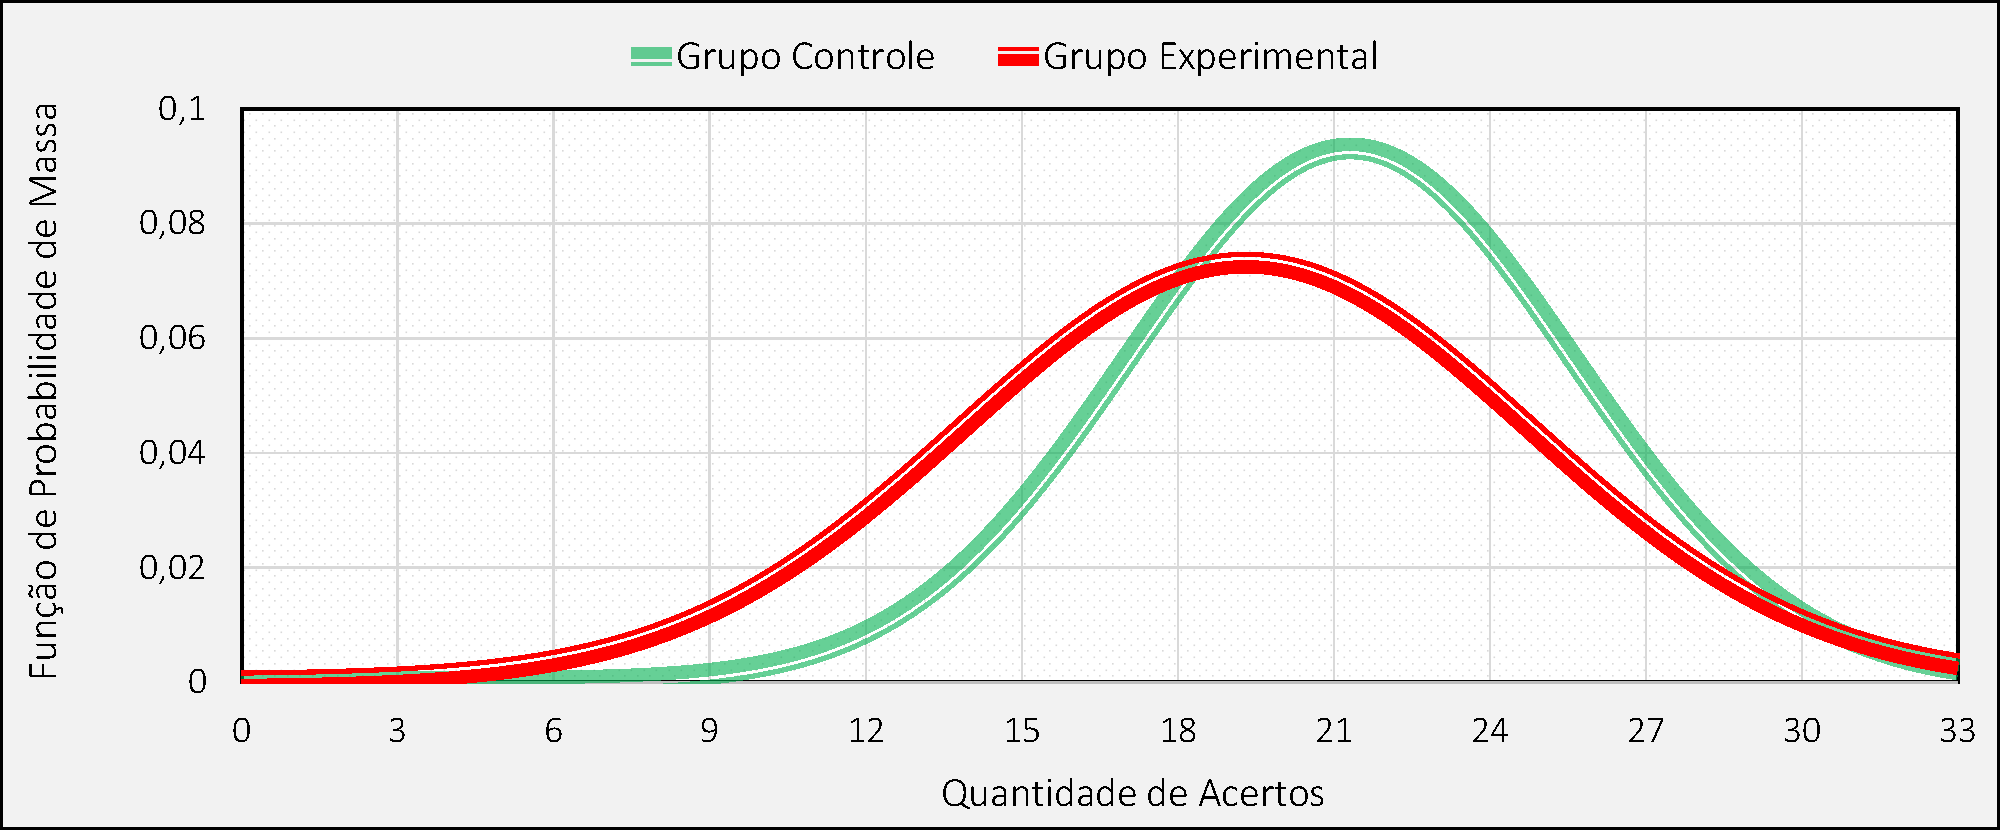
\includegraphics[width=\linewidth]{./Visuais/GraficosPosteste.pdf}
    \legend{Fonte: Elaborada pelo autor (2021).}
\end{figure}


O Teste \textit{t} mostrou que não há diferenças significativas entre as médias das amostras (t$_{(27)}$ = 1,109; p = 0,27697). Ou seja, os resultados do Teste \textit{t} indicam não haver diferenças de conhecimento entre as crianças do grupo controle e as crianças do grupo experimental, no que diz respeito aos conhecimentos medidos pelo instrumento avaliativo \ac{CKAQ}. Desta forma a hipótese nula (H$_0$) do Teste \textit{t} deve ser aceita, indicando que não existem diferenças entre as médias das amostras ($\mu$$_{controle}$ = $\mu$$_{experimental}$). %Os máximos globais de cada grupo, são as médias já calculadas e ilustradas na \autoref{fig:caixapre1}. 
Um comparativo da evolução de desempenho dos grupos entre o pré e o pós-teste pode ser observado na \autoref{fig:normal2}.

\begin{figure}[htb]
    \centering
    \caption{\label{fig:normal2}Distribuição comparativa, pré-teste e pós-teste.}
    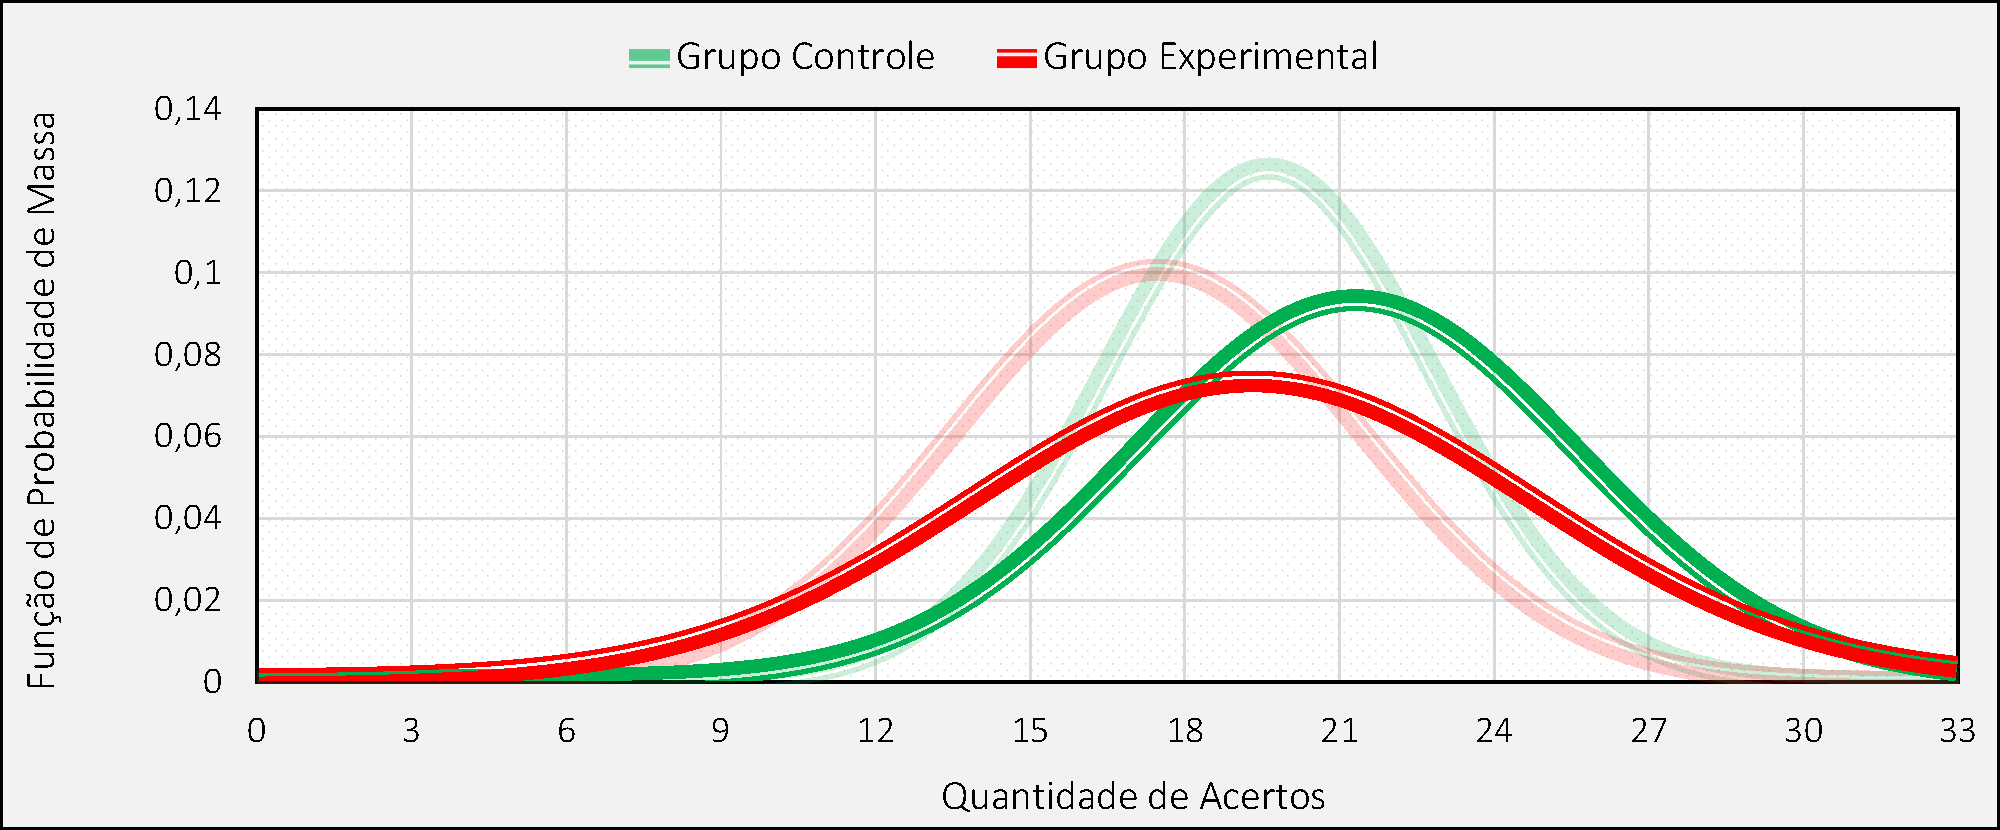
\includegraphics[width=\linewidth]{./Visuais/GraficosAntesDepois.pdf}
    \legend{Fonte: Elaborada pelo autor (2021).}
\end{figure}

A \autoref{fig:normal2} apresenta as curvas normais de ambos os grupos estudados. De forma mais nítidas são representadas as curvas da etapa de pós-teste, as demais curvas representam a etapa de pré-teste. Comparando o pré com o pós-teste é possível constatar que ambas as curvas ficaram mais achatadas, indicando uma maior dispersão da quantidade de questões acertadas. 

Os resultados alcançados nessa seção apontam; tanto para uma média, quanto para uma mediana, equivalente entre as amostras. Sendo assim, a \hyperref[hipotese]{hipótese nula} (H$_0$) da corrente pesquisa deve ser aceita, rejeitando-se a hipótese alternativa (H$_1$). Desta forma é possível inferir com um grau de confiança de 95\% que o programa educacional desenvolvido nessa pesquisa não foi capaz de influenciar estatisticamente o grupo experimental (nem positivamente, nem negativamente). Ou seja, o jogo desenvolvido pela presente pesquisa não aparenta ter interferido estatisticamente no conhecimento das crianças do grupo experimental em relação aos conhecimentos do grupo controle no que diz respeito aos conhecimentos medidos pelo instrumento avaliativo \ac{CKAQ}. As implicações sobre esse resultado são deliberadas mais detalhadamente na \autoref{ch:Conclusao} do presente trabalho acadêmico.

Uma vez constatada a equivalência das médias e das medianas entre os grupos, a atual pesquisa se dispôs a calcular também, suas relações internas, comparando os resultados pareados na etapa de pré-teste em comparação a etapa de pós-teste. Além disso, a corrente pesquisa também buscou identificar possíveis relações entre o desempenho das crianças no jogo e suas pontuações atingidas no questionário \ac{CKAQ}. Nesse sentido, observou-se que o jogador com o melhor desempenho no jogo, obteve uma pontuação média no questionário de 17 (dezessete) acertos. Por tal razão, não é possível estabelecer qualquer relação entre o jogo desenvolvido por essa pesquisa e o questionário aplicado. 

%O presente estudo também se dispós a medir a relação interna do grupo experimental, verificando não apenas seu desempenho na etapa de pré-teste em relação etapa de pós-teste, mas também encontrar possíveis relações de desemenho no jogar dos jogo pelas crianças (o presente estudo também relaciona as variáveis de desempenho e aprendizagem a fim de encontrar relações entre o desempenho de determinados indivíduos em um jogo e o aprimoramento de suas habilidades intelectuais no que diz respeito aos assuntos ministrados pelo jogo.) Nesse sentido, observou-se que a criança com a menor taxa de erros durante os teste com o jogo, foi a criança com menor desempenho no questionário (12 acertos). E a criança com a maior taxa de acertos durante os testes com o jogo, teve um desempenho médio no questionário (17 acertos). Por tal razão, nada se pode afirmar sobre uma possivel associação entre o desempenho das crianças no jogo e seu desempenho no questionario. Nenhuma relação foi identificada, portanto nenhum gráfico ou estatísticas foram gerados. 

As relações internas do grupo experimental foram calculadas com auxílio do Teste \textit{t} e do teste de \textit{Wilcoxon}. O teste de \textit{Wilcoxon} é um teste para amostras relacionadas, usado para comparar suas medianas. Os cálculos com o teste de \textit{Wilcoxon} apontaram que as medianas entre o pré e o pós-teste do grupo experimental são de fato equivalentes (z = 1,06312; p = 0,30127). Desta forma a hipótese nula (H$_0$) do teste de \textit{Wilcoxon} deve ser aceita, indicando com 95\% de confiança de que as medianas são equivalantes (\textit{M}$_{pr\acute{e}-experimental}$ = \textit{M}$_{p\acute{o}s-experimental}$). 

O Teste \textit{t} para amostras relacionadas mostrou que não há diferenças significativas de conhecimento entre o pré e pós-teste do grupo experimental, no que tange os conhecimentos medidos pelo instrumento avaliativo \ac{CKAQ} (t$_{(12)}$ = -1,38873; p = 0,19015). Desta forma a hipótese nula (H$_0$) do Teste \textit{t} deve ser aceita, indicando que não existe diferenças significativas ($\alpha$ = 5\%) entre as médias ($\mu$$_{pr\acute{e}-experimental}$ = $\mu$$_{p\acute{o}s-experimental}$).

Os resultados alcançados nessa seção apontam; tanto para uma média, quanto para uma mediana, equivalente entre as amostras (e entre as etapas de pré e pós-teste para o grupo experimental). Notoriamente, os cálculos matemáticos realizados pela presente pesquisa não estão isentos de falhas, portanto, com intuito de facilitar a revisão dos resultados alcançados, e com intuito de deixar todo o processo mais transparente o possível a corrente pesquisa publica todos os dados obtidos nessa etapa no \autoref{chap:resul2}.


\section{Apreciação}\label{sec:apreciar}

A etapa de apreciação do corrente trabalho foi conduzida no dia 22 (vinte e dois) de novembro de 2021 às 14h20 (hora local). A etapa de apreciação surge na presente pesquisa com o objetivo de identificar os índices de satisfação das crianças que jogaram o jogo desenvolvido, por tal razão tal etapa é realizada apenas com as crianças do grupo experimental. A medição foi realizada com uma versão adaptada (\autoref{chap:Apreciacao}) do \acf{MEEGA}.

O grupo experimental participou da etapa de apreciação do atual trabalho sob as mesmas condições a qual foram submetidos na etapa de pós-teste (\autoref{sec:postes}), inclusive a etapa de apreciação teve início imediato, ao término da etapa de pós-teste. O processo como um todo contou com a participação de 13 (treze) crianças e durou trinta minutos, finalizando às 15h50 (hora local). Em um primeiro momento, foi entregue uma cópia impressa do \ac{MEEGA} adaptado a todas as crianças. Os dados quantitativos da presente etapa são apresentados na \autoref{fig:barrasNOTAS}

\begin{figure}[htb]
    \caption{\label{fig:barrasNOTAS}Taxa de satisfação por questão, grupo experimental.}
    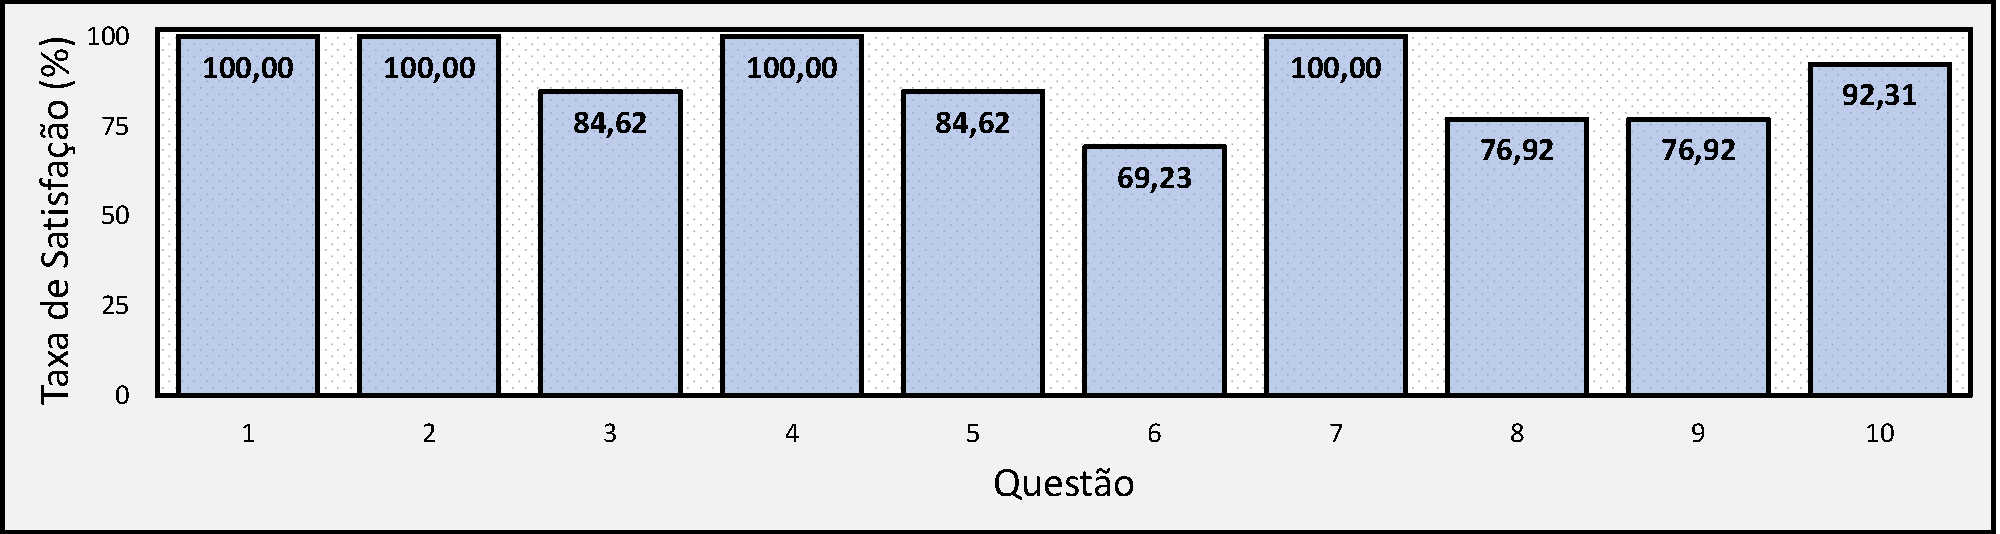
\includegraphics[width=\linewidth]{./Visuais/NotasTaxa.pdf}
    \legend{Fonte: Elaborada pelo autor (2021).}
\end{figure}

A \autoref{fig:barrasNOTAS} ilustra no eixo das abscissas o número da questão do questionário \ac{MEEGA} adaptado e no eixo das ordenadas a taxa de satisfação para aquela determinada questão. O somatório dos itens do questionário \ac{MEEGA} adaptado apontou para uma nota de satisfação normalizada de 9,192 (os itens são medidos conforme a escala \textit{Likert} de -1 até +1). Tal valor se aproxima da nota média dada pelas crianças 9,25 (última questão do questionário). Notoriamente, os cálculos matemáticos realizados pela presente pesquisa não estão issentos de falhas, portanto, com intuito de facilitar a revisão dos resultados alcançados, e com intuito de deixar todo o processo mais transparente o possível a corrente pesquisa pública todos os dados obtidos nessa etapa no \autoref{chap:resul3}.

Após a aplicação do questionário \ac{MEEGA}, iniciou-se um grupo focal com as crianças, fornecendo espaço para se manifestarem livremente e deliberarem sobre o jogo, apontado suas principais satisfações e angústias. As observações, ideias e sugestões apontadas pelas crianças são descritas no \autoref{ch:Conclusao} do presente trabalho acadêmico, de modo a compilar conjuntamente as ideias manifestadas pelos profissionais envolvidos na corrente pesquisa.



\section{Análise Comparativa}\label{sec:compilar}

Os resultados alcançados pela presente pesquisa apontam para uma equivalência estatística entre os grupos estudados, tanto em termos de suas médias, quanto de suas medianas. Sendo assim, o grupo experimental não demonstra qualquer diferença estatística com o grupo controle (levando em consideração as variáveis mensuradas). Um comparativo com demais trabalhos na área é apresentado na \autoref{tab-nivinv2}.

\newcolumntype{P}[1]{>{\centering\arraybackslash}p{#1}}
\newcolumntype{M}[1]{>{\centering\arraybackslash}m{#1}}
\begin{table}[htb]
\footnotesize
\renewcommand{\arraystretch}{1.5} %espaço entre as linhas
\caption[Comparativo entre os Trabalhos Relacionados e o Atual Trabalho.]{Comparativo entre os Trabalhos Relacionados e o Atual Trabalho.}
\label{tab-nivinv2}
\centering
\begin{tabular}{p{4.2cm}p{2.0cm}M{2.2cm}M{1.5cm}M{2.0cm}M{2.1cm}}
  \toprule
   \textbf{Jogo (Ano)} & \textbf{Idioma}  & \textbf{Público-alvo} & \textbf{Amostra} & \multicolumn{2}{c}{\textbf{Validação (pós-teste)}}  \\
   \cline{5-6}
     &  &  &  & Grupo Controle & Grupo Experimental\\
   \midrule
    \textit{Being Safety Smart} (2009)  & Inglês          & 6-8 anos    & 76    & \textcolor[rgb]{0.9,0,0}{\textbf{69\%}}      & \textcolor[rgb]{0,0.6,0}{\textbf{90\%}} \\
    \hline
    \textit{Orbit Rescue} (2012)        & Inglês          & 8-10 anos   & 139    & \textcolor[rgb]{0.9,0,0}{\textbf{75\%}}      & \textcolor[rgb]{0,0.6,0}{\textbf{93\%}} \\
    \hline
    \textit{Cool and Safe} (2013)       & $\tfrac{Alem\tilde{a}o/Franc\hat{e}s}{Ingl\hat{e}s/Espanhol}$  & 7-12 anos   & 286   & \textcolor[rgb]{0.9,0,0}{\textbf{61\%}}      & \textcolor[rgb]{0,0.6,0}{\textbf{79\%}} \\
    \hline
    \textit{Infância Segura} (2021)     & $\tfrac{Portugu\hat{e}s}{Espanhol/Ingl\hat{e}s}$       & 5-8 anos    & 33      &   \textcolor[rgb]{0.7,0.7,0}{\textbf{65\%}}       &   \textcolor[rgb]{0.7,0.7,0}{\textbf{58\%}}  \\
    \hline
    \bottomrule
\end{tabular}
\legend{Fonte: Elaborada pelo autor (2021).}
\end{table}

A \autoref{tab-nivinv2} realiza um comparativo entre diferentes jogos voltados a prevenção da violência sexual infantil. A distribuição dos itens na tabela segue de maneira equivalente a da \autoref{tab-nivinv}, tendo como único diferencial, a inclusão de mais um jogo. É possível observar na \autoref{tab-nivinv2} que todas as propostas de jogos do exterior, demonstram-se promissoras no ensino de habilidades preventivas no que diz respeito aos itens medidos pelo instrumento avaliativo \ac{CKAQ}. A proposta nacional falha em demonstrar resultados estatísticos aceitáveis. 

Ao se tratar dos métodos estatísticos, é importante salientar que, devido a natureza distinta dos dados, cada pesquisa se utilizou de métricas estatísticas próprias para a conclusão de seus resultados. Por tal razão, é fundamental deixar claro que os valores apresentados foram normalizados para proporcionar uma comparação mais clara entre os resultados alcançados por cada pesquisa. 

A corrente pesquisa iniciou uma abordagem com 112 (cento e doze crianças), todavia apenas 33 (trinta e três) apresentaram documentação necessária para participar das etapas do atual trabalho. No mais, é importante deixar claro que, embora a taxa média de acerto do grupo controle (65\%) seja superior a taxa média de acerto grupo experimental (58\%), os dados estatísticos são robustos o suficiente para afirmar que não há diferenças significativas entre as amostras com uma taxa de confianças de 95\%. Salienta-se, inclusive que ambos os grupos apresentaram melhora nos seus desempenhos, quando comparados seus resultados isolados no pré e no pós-teste. Todavia, suas melhoras também não apresentam qualquer diferença estatística (nem para o grupo controle, nem para o grupo experimental). A conclusão dos resultados é apresentada detalhadamente no \autoref{ch:Conclusao}.
